% Fig 2: structures of the frozen models (results/final.pt; PROJECT_PLAN.md section 5).
% (a) ReLU MLP, 3 layers: 4 inputs -> 50 ReLU -> 2 linear outputs, 352 weights.
% (b) KBNN, 4 layers: parameter block z -> 25 ReLU -> (t0, tau, E0, s); correction block (v, z) -> 25 ReLU -> (g, q),
%     minus its value at v = 0; softplus on tau and s (state in the caption); knowledge layer: the log-law
%     formulas (no weights). 381 weights.
% Build: pdflatex fig2_structures.tex (output copied to ../figs/)
\documentclass[border=4pt]{standalone}
\usepackage{tikz}
\usepackage{amsmath}
\usepackage{helvet}
\renewcommand{\familydefault}{\sfdefault}
\usetikzlibrary{positioning, calc, arrows.meta, fit, backgrounds}
\definecolor{mlp}{HTML}{EB6834}
\definecolor{kbnn}{HTML}{2A78D6}
\definecolor{ink2}{HTML}{52514E}
\definecolor{edge}{HTML}{C3C2B7}
\definecolor{shade}{HTML}{F0EFEC}
\begin{document}
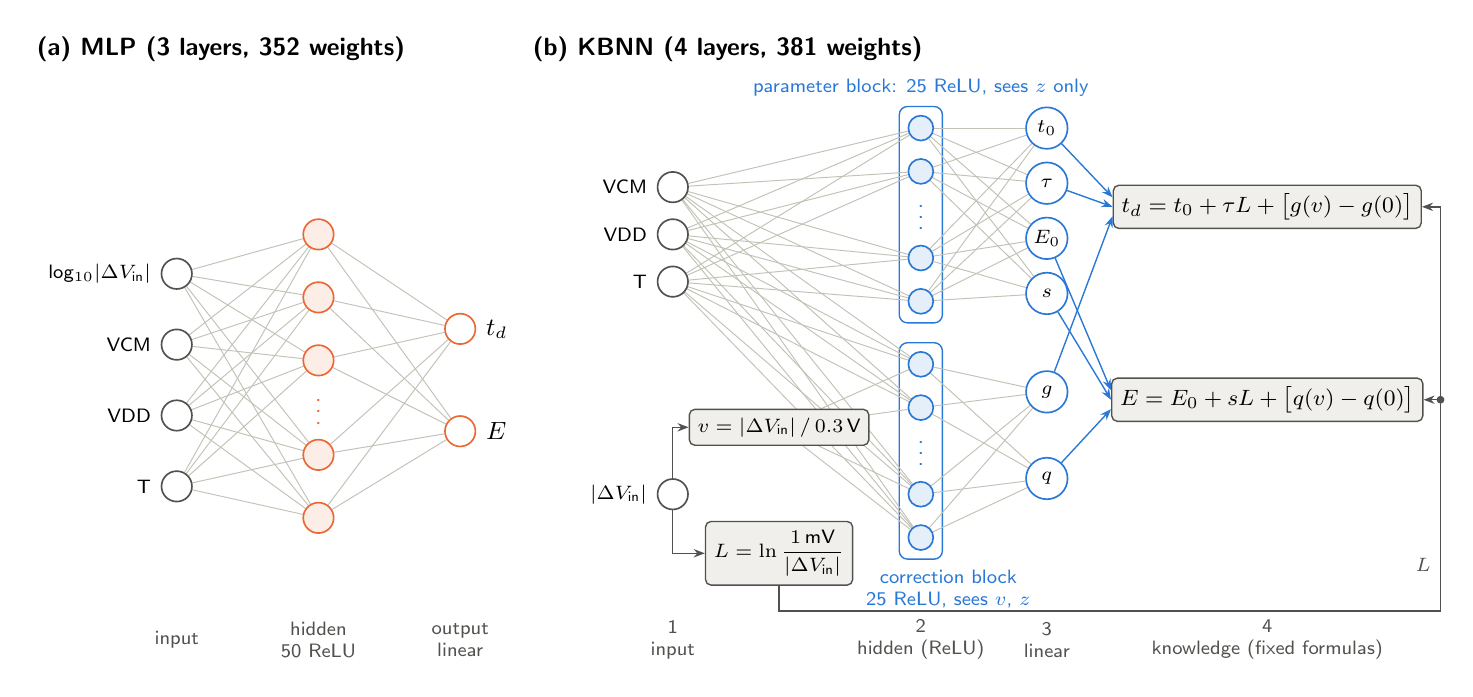
\begin{tikzpicture}[font=\footnotesize, >={Stealth[length=4pt]},
    neuron/.style={circle, draw, line width=0.6pt, minimum size=11pt, inner sep=0},
    io/.style={circle, draw=ink2, fill=white, line width=0.6pt, minimum size=11pt, inner sep=0},
    lin/.style={circle, draw=#1, fill=white, line width=0.6pt, minimum size=11pt, inner sep=0},
    fixed/.style={rounded corners=2pt, draw=ink2, fill=shade, line width=0.5pt, inner sep=3pt, align=left},
    w/.style={edge, line width=0.35pt}, layer/.style={font=\scriptsize, text=ink2, align=center}]

% ============================== (a) MLP ==============================
\begin{scope}[shift={(0,0)}]
  \node[font=\small\bfseries, anchor=west] at (-1.9,6.75) {(a) MLP (3 layers, 352 weights)};
  \foreach \y/\t [count=\i] in {3.9/{log$_{10}|\Delta V_\text{in}|$}, 3.0/VCM, 2.1/VDD, 1.2/T}
    \node[io, label={[font=\scriptsize]left:\t}] (a\i) at (0,\y) {};
  \foreach \y [count=\i] in {4.4, 3.6, 2.8, 1.6, 0.8}
    \node[neuron, draw=mlp, fill=mlp!12] (h\i) at (1.8,\y) {};
  \node[text=mlp] at (1.8,2.25) {$\vdots$};
  \foreach \y/\t [count=\i] in {3.2/$t_d$, 1.9/$E$}
    \node[lin=mlp, label={[font=\small]right:\t}] (o\i) at (3.6,\y) {};
  \begin{scope}[on background layer]
    \foreach \i in {1,...,4} \foreach \j in {1,...,5} \draw[w] (a\i) -- (h\j);
    \foreach \j in {1,...,5} \foreach \k in {1,2} \draw[w] (h\j) -- (o\k);
  \end{scope}
  \node[layer] at (0,-0.75) {input};
  \node[layer] at (1.8,-0.75) {hidden\\50 ReLU};
  \node[layer] at (3.6,-0.75) {output\\linear};
\end{scope}

% ============================== (b) KBNN ==============================
\begin{scope}[shift={(6.3,0)}]
  \node[font=\small\bfseries, anchor=west] at (-1.9,6.75) {(b) KBNN (4 layers, 381 weights)};
  % layer 1: inputs z = (VCM, VDD, T) and |dVin|
  \foreach \y/\t [count=\i] in {5.0/VCM, 4.4/VDD, 3.8/T}
    \node[io, label={[font=\scriptsize]left:\t}] (z\i) at (0,\y) {};
  \node[io, label={[font=\scriptsize]left:$|\Delta V_\text{in}|$}] (dv) at (0,1.1) {};
  % fixed input transforms (no weights)
  \node[fixed, font=\scriptsize] (v) at (1.35,1.95) {$v = |\Delta V_\text{in}|\,/\,0.3$\,V};
  \node[fixed, font=\scriptsize] (L) at (1.35,0.35) {$L = \ln\dfrac{1\,\text{mV}}{|\Delta V_\text{in}|}$};
  \draw[->, ink2, line width=0.5pt] (dv) |- (v);
  \draw[->, ink2, line width=0.5pt] (dv) |- (L);
  % layer 2: two ReLU blocks
  \foreach \y [count=\i] in {5.75, 5.2, 4.1, 3.55}
    \node[neuron, draw=kbnn, fill=kbnn!12, minimum size=9pt] (p\i) at (3.15,\y) {};
  \node[text=kbnn] at (3.15,4.72) {$\vdots$};
  \foreach \y [count=\i] in {2.75, 2.2, 1.1, 0.55}
    \node[neuron, draw=kbnn, fill=kbnn!12, minimum size=9pt] (c\i) at (3.15,\y) {};
  \node[text=kbnn] at (3.15,1.72) {$\vdots$};
  \begin{scope}[on background layer]
    \node[draw=kbnn, rounded corners=3pt, line width=0.5pt, fit=(p1)(p4), inner sep=3pt] (PB) {};
    \node[draw=kbnn, rounded corners=3pt, line width=0.5pt, fit=(c1)(c4), inner sep=3pt] (CB) {};
    \foreach \i in {1,2,3} \foreach \j in {1,...,4} \draw[w] (z\i) -- (p\j);
    \foreach \i in {1,2,3} \foreach \j in {1,...,4} \draw[w] (z\i) -- (c\j);
    \foreach \j in {1,...,4} \draw[w] (v) -- (c\j);
  \end{scope}
  \node[font=\scriptsize, text=kbnn, anchor=south] at (PB.north) {parameter block: 25 ReLU, sees $z$ only};
  \node[font=\scriptsize, text=kbnn, anchor=north, align=center] at ($(CB.south)+(0.35,0)$) {correction block\\25 ReLU, sees $v$, $z$};
  % layer 3: linear outputs (softplus keeps tau and s positive)
  \foreach \y/\t [count=\i] in {5.75/t_0, 5.05/\tau, 4.35/E_0, 3.65/s}
    \node[lin=kbnn, minimum size=15pt, font=\scriptsize] (q\i) at (4.75,\y) {$\t$};
  \foreach \y/\t [count=\i] in {2.4/g, 1.3/q}
    \node[lin=kbnn, minimum size=15pt, font=\scriptsize] (r\i) at (4.75,\y) {$\t$};
  \begin{scope}[on background layer]
    \foreach \j in {1,...,4} \foreach \k in {1,...,4} \draw[w] (p\j) -- (q\k);
    \foreach \j in {1,...,4} \foreach \k in {1,2} \draw[w] (c\j) -- (r\k);
  \end{scope}
  % layer 4: knowledge layer, fixed formulas
  \node[fixed, font=\footnotesize] (kt) at (7.55,4.75) {$t_d = t_0 + \tau L + \bigl[g(v) - g(0)\bigr]$};
  \node[fixed, font=\footnotesize] (ke) at (7.55,2.3) {$E = E_0 + s L + \bigl[q(v) - q(0)\bigr]$};
  \foreach \a/\b in {q1/0.12, q2/0, r1/-0.12} \draw[->, kbnn, line width=0.5pt] (\a) -- ($(kt.west)+(0,\b)$);
  \foreach \a/\b in {q3/0.12, q4/0, r2/-0.12} \draw[->, kbnn, line width=0.5pt] (\a) -- ($(ke.west)+(0,\b)$);
  % L into both formulas, routed below and up the right side
  \draw[ink2, line width=0.5pt] (L.south) -- ++(0,-0.32) coordinate (Lb) -- (Lb -| 9.75,0) coordinate (Lr);
  \draw[->, ink2, line width=0.5pt] (Lr) |- (ke.east);
  \draw[->, ink2, line width=0.5pt] (ke.east -| Lr) node[circle, fill=ink2, inner sep=1pt] {} |- (kt.east);
  \node[font=\scriptsize, text=ink2, anchor=south east] at (Lr |- 0,0.0) {$L$};
  % layer labels
  \node[layer] at (0,-0.75) {1\\input};
  \node[layer] at (3.15,-0.75) {2\\hidden (ReLU)};
  \node[layer] at (4.75,-0.75) {3\\linear};
  \node[layer] at (7.55,-0.75) {4\\knowledge (fixed formulas)};
\end{scope}
\end{tikzpicture}
\end{document}
